\documentclass{standalone}

\usepackage{tikz}
\usetikzlibrary{arrows,er,shapes,fit,chains}

\begin{document}
  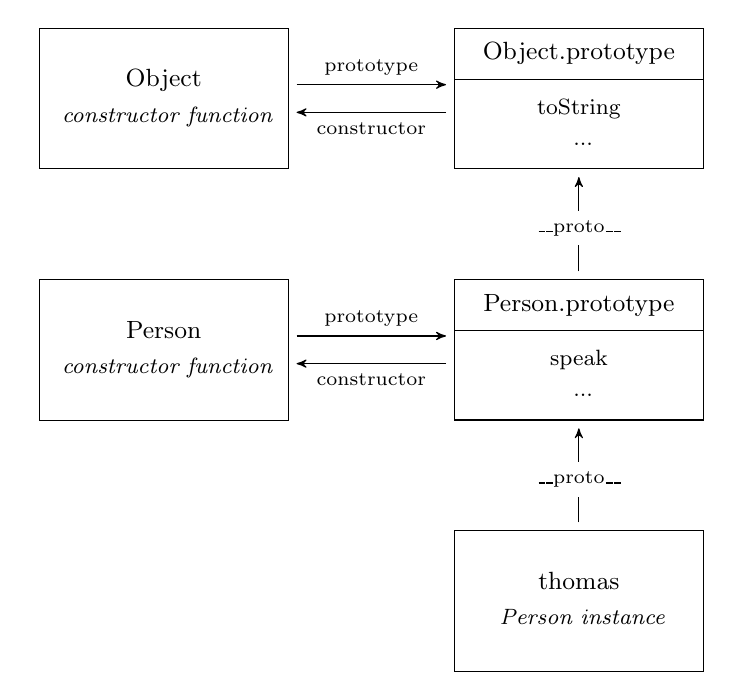
\begin{tikzpicture}[
  ->,
  >=stealth',
  shorten >= 1pt,
  auto,
  node distance=4em and 6em,
  font=\small,
  text centered,
  every entity/.style={
    minimum width=9em,
    outer sep=0,
    inner ysep=.5em
  }
  ]
  
  \node [entity] (B) [rectangle split, rectangle split parts=2, text centered] {
  Object.prototype \nodepart{two} \begin{tabular}{c}\footnotesize{toString} \\ \footnotesize{...}\end{tabular}
  };

  \node [entity] (A) [fit=(B), left = of B, inner sep=0] {};
  \node at (A.center) {\begin{tabular}{c}Object \\[.2em] \footnotesize{\emph{constructor function}}\end{tabular}};

  \node [entity] (C) [fit=(B), below = of A, inner sep=0] {};
  \node at (C.center) {\begin{tabular}{c}Person \\[.2em] \footnotesize{\emph{constructor function}}\end{tabular}};

  \node [entity] (D) [right = of C] [rectangle split, rectangle split parts=2, text centered] {
  Person.prototype \nodepart{two} \begin{tabular}{c}\footnotesize{speak} \\ \footnotesize{...}\end{tabular}
  };

  \node [entity] (E) [fit=(B), below = of D, inner sep=0] {};
  \node at (E.center) {\begin{tabular}{c}thomas \\[.2em] \footnotesize{\emph{Person instance}}\end{tabular}};


  \path[shorten >=0.3em,shorten <=0.3em,->] ([yshift=0.5em]A.east) edge node {\scriptsize{prototype}} ([yshift=0.5em]B.west);
  \path[shorten >=0.3em,shorten <=0.3em,->] ([yshift=-0.5em]B.west) edge node {\scriptsize{constructor}} ([yshift=-0.5em]A.east);

  \path[shorten >=0.3em,shorten <=0.3em,->] ([yshift=0.5em]C.east) edge node {\scriptsize{prototype}} ([yshift=0.5em]D.west);
  \path[shorten >=0.3em,shorten <=0.3em,->] ([yshift=-0.5em]D.west) edge node {\scriptsize{constructor}} ([yshift=-0.5em]C.east);

  \path[shorten >=0.3em,shorten <=0.3em,->] (E) edge node[anchor=center, fill=white, yshift=-0.15em] {\scriptsize{\_\_proto\_\_}} (D);
  \path[shorten >=0.3em,shorten <=0.3em,->] (D) edge node[anchor=center, fill=white, yshift=-0.15em] {\scriptsize{\_\_proto\_\_}} (B);
  
  \end{tikzpicture}
\end{document}